\documentclass[a4paper,11pt]{book}

% packages de base
\usepackage[french]{babel}
\usepackage[utf8]{inputenc}
\usepackage[T1]{fontenc}

% packages additionnels
\usepackage[top=4cm, bottom=4cm, left=3cm, right=3cm]{geometry}  % Pour redimensionner les marges
\usepackage{graphicx}  % Pour les figures
\usepackage{url}  % Pour l'insertion des url

% Titre du livre
\title{Surfer sur le \\ \texttt{World Wide Web} \\ avec \\ \texttt{Mozilla Firefox}}
\author{Krystof2so}
\date{\today}

\begin{document}
\maketitle
\frontmatter
\chapter*{Présentation générale}
\section*{\texttt{Mozilla Firefox}}
Un navigateur sert à arpenter le \textit{web}. \texttt{Mozilla Firefox} est un navigateur \textit{web}libre conçu par la \textit{Fondation Mozilla}\footnote{\url{https://www.mozilla.org/fr/}} depuis 2003, et depuis 2005, c'est l'entreprise \textit{Mozilla Corporation}\footnote{\url{https://en.wikipedia.org/wiki/Mozilla_Corporation}} qui est chargée de son développement. \texttt{Firefox} est disponible sous licence libre \textit{Mozilla Public License} (\textit{MPL})\footnote{\url{https://www.gnu.org/licenses/license-list.fr.html#MPL-2.0}}.
\medskip

Jusqu'en 2010, \texttt{Mozila Firefox} a connu un fort essor avant de voir sa part de marché diminuer au profit du navigateur développé par \textit{Google} qu'est \texttt{Google Chrome}.
\medskip

Il s'agit d'un navigateur complet, et ce grâce à de nombreux modules complémentaires que l'on peut lui rajouter. Il est fréquemment installé par défaut sur de nombreuses distributions \textit{GNU/Linux}.
\medskip

\texttt{Firefox} propose tout ce que l’on peut attendre d’un navigateur moderne : gestion des onglets, navigation privée, envoi de sites vers d’autres appareils connectés, synchronisation des données, enregistrement des mots de passe, ou bien encore l’extraction d’une vidéo dans une fenêtre séparée, ainsi que divers thèmes graphiques. Il est également reconnu comme étant un des plus sécurisés\footnote{En 2019, l'agence allemande de sécurité informatique (\textit{BSI}) recommande \texttt{Firefox}, considérant qu'il est le navigateur le plus sécurisé.}.
\medskip

\section*{La vie privée}
Sans être le navigateur le plus radicale en la matière, \texttt{Firefox} se montre proactif en ce qui concerne le respect de la vie privée\footnote{Politique de confidentialité avec \texttt{Firefox}: \url{https://www.mozilla.org/fr/privacy/firefox/}}, qui devient au fil des années son argument majeur. En effet, \texttt{Firefox}, dans son paramétrage inclut trois niveaux de protection (\textit{standard}, \textit{strict} et \textit{personnalisé}).
\medskip

Par défaut les traqueurs du \textit{Web} sont bloqués:
\begin{itemize}
	\item traqueurs de réseaux sociaux;
	\item cookies intersites;
	\item contenu utilisé pour le pistage dans toutes les fenêtres;
	\item mineurs de cryptomonnaies;
	\item détecteurs d’empreinte numérique.
\end{itemize} 
\medskip

\section*{Les fonctionnalités natives}
\begin{itemize}
	\item la navigation par onglets;
    \item un bloqueur de fenêtres intruses (appelées aussi \textit{pop-ups});
    \item des marque-pages (appelés \og favoris\fg{} ou \og signets\fg{} dans les navigateurs concurrents); 
    \item un gestionnaire de téléchargement;
    \item un correcteur orthographique intégré;
    \item un filtre anti-hameçonnage (\og filoutage\fg{} ou \textit{phishing});
    \item un mode de navigation privée par fenêtre, où \texttt{Firefox} ne conserve aucune donnée sur les sites et pages visités;
    \item la navigation avec géolocalisation intégrée;
    \item un lecteur de \textit{PDF} intégré;
    \item un mode lecture;
    \item un service intégré de lecture différée multiplateforme (\texttt{Pocket}, racheté par \textit{Mozilla Foundation} en février 2017);
    \item un outil de capture d'écran depuis le 28 septembre 2017, qui propose pour principale innovation la sélection automatique des éléments de la page;
    \item un outil de synchronisation \texttt{Firefox Sync} qui permet de synchroniser les marque-pages, l'historique de navigation, les préférences, les mots de passe et les derniers onglets ouverts à travers différents appareils;
    \item des outils de développement web (analyse de code source, script, etc.);
    \item le \textit{DNS over HTTPS} (\textit{DoH}).
\end{itemize}
\medskip

\section*{Les extensions: l'autre atout}
Les extensions permettent d’ajouter de nouvelles fonctionnalités au navigateur, comme la météo, un blocage des publicités des sites \textit{Web}, des outils de développement \textit{Web}, etc. Elles permettent également de changer son apparence (grâce aux thèmes).
\medskip

Les extension souvent recommandées sont avant tout liées à la vie privée.
\medskip

\section*{Personnalisation et paramétrage}
\texttt{Firefox} dispose d’un panneau d’options permettant de configurer une grande partie du navigateur. Le fait de taper \texttt{about:config} dans la barre d’adresse permet d’accéder à des paramètres avancés et configurer de nombreux éléments.
\medskip

\section*{Des versions diverses}
\texttt{Firefox} est un logiciel en développement continu. Et il existe différentes versions qui sont développées en parallèle des unes des autres. Une version donnée de \texttt{Firefox} passera par ce processus : \textit{Nightly → Developer Edition} ou \textit{Beta → Version finale stable}. C'est sur \textit{Nightly} que sont implémentées les nouvelles fonctionnalités, \textit{Developper Edition} et \textit{Beta} sont des versions intermédiaires permettant de figer les fonctionnalités pour stabiliser le code et corriger les bugs avant de devenir la version stable.
\medskip

Depuis 2012, \texttt{Firefox} dispose d'une édition \texttt{ESR} (\textit{Extended Support Release}), qui garantit au moins un an de support technique. Contrairement à la mouture classique où le support ne vaut que pour la version en cours, \texttt{Firefox ESR} est \og bloqué\fg{} pendant un an. Le socle fonctionnel ne change pas, mais les failles de sécurité sont corrigées. Un chevauchement de 43 semaines est prévu entre deux versions \texttt{ESR}.
\medskip

De plus \texttt{Firefox} sert de bases à divers projets, à l'instar de celui de \texttt{Tor Browser}\footnote{\url{https://www.torproject.org/download/}} (basé sur la version \texttt{ESR}).
\medskip

\mainmatter
\chapter{Installation}
\section{Configuration du navigateur}
\subsection*{Personnaliser le menu ou la barre d'outils}\label{barre_outils}
\begin{verbatim}
    Bouton "Menu" > Outils supplémentaires > Personnaliser la barre 
    d'outils...
\end{verbatim}
\medskip

\begin{figure}[h]
\begin{center}
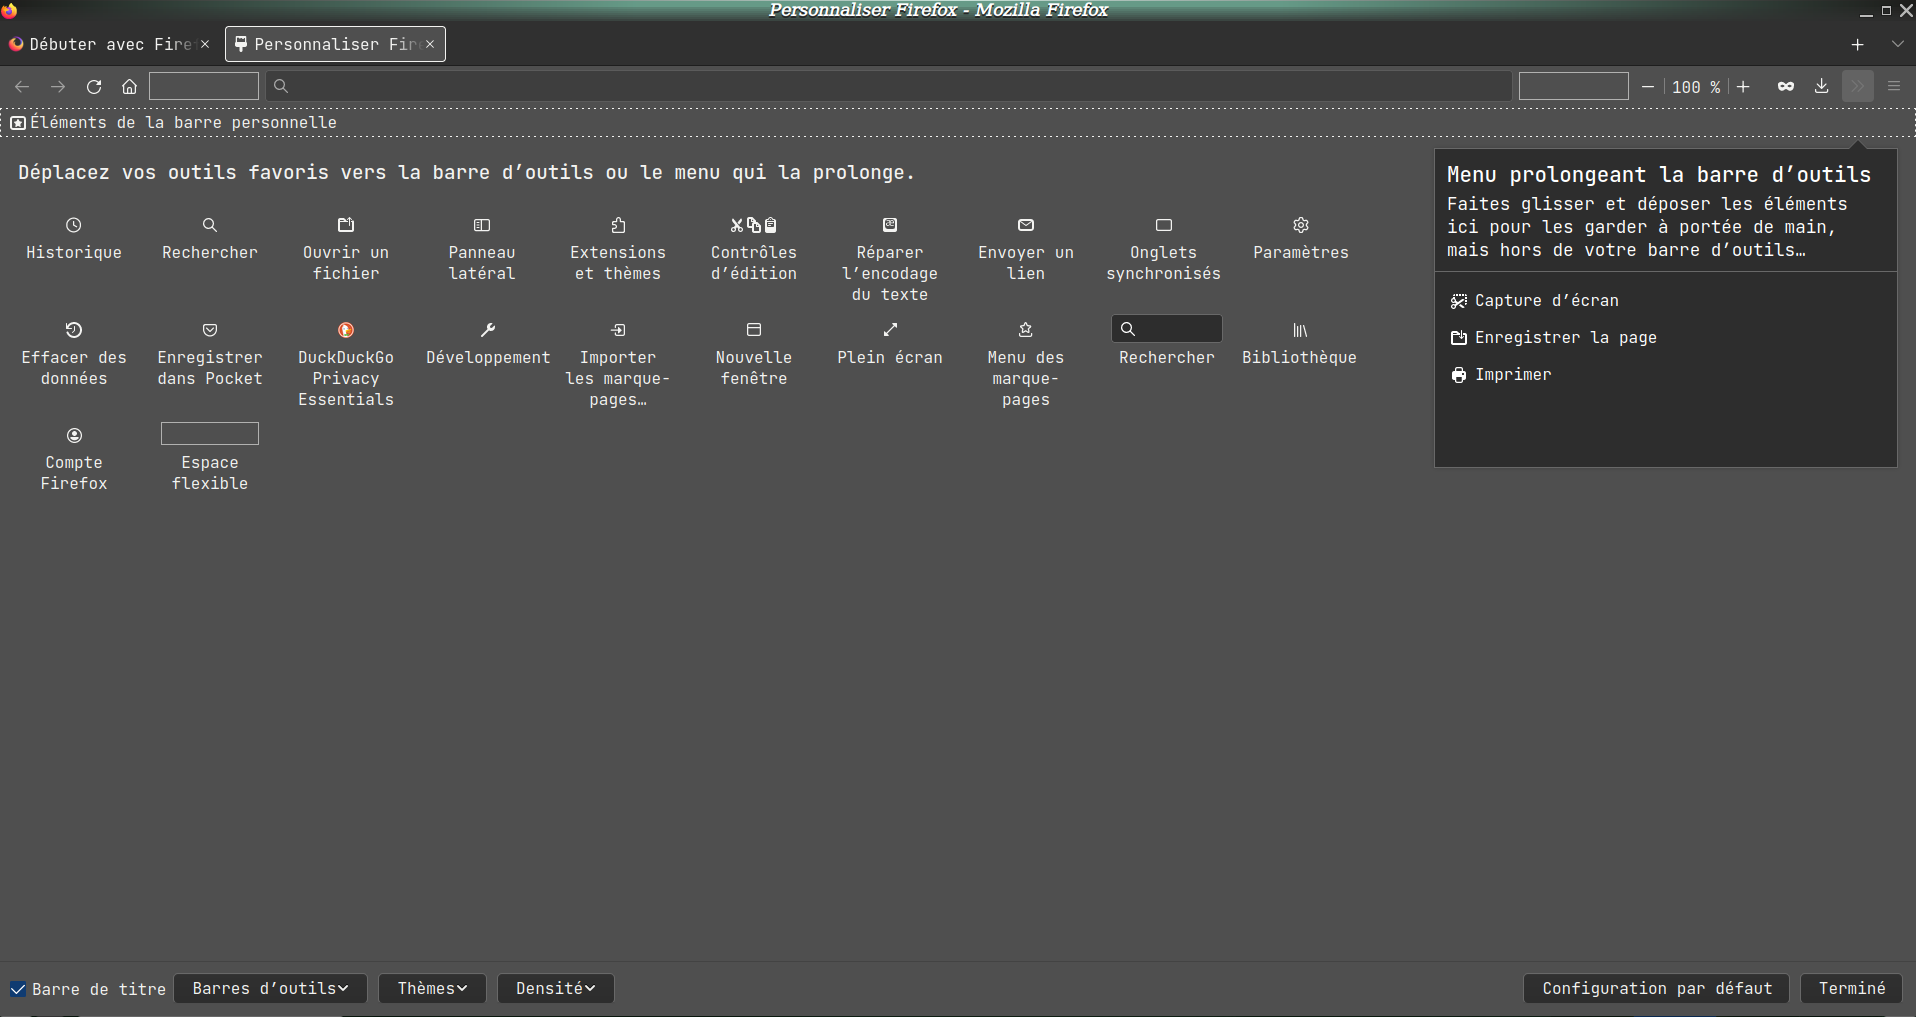
\includegraphics[scale=0.2]{IMG/003--Ecran.png}
\caption{Personnaliser la barre d'outils}
\end{center}
\end{figure}
\medskip

Ensuite, glissez-déposez les fonctionnalités que vous souhaitez dans votre barre d’outils ou sur le panneau de droite. 
\medskip



\chapter{Naviguer avec \texttt{Firefox}}
\section{La page d'accueil}
Il est possible de configurer la page d'accueil (ou \textit{page de nouvel onglet}) afin que quand on lance \texttt{Firefox}, ou que l'on ouvre un nouvel onglet, ce soit la page voulue par défaut qui s'ouvre systématiquement.
\begin{figure}[h]
\begin{center}
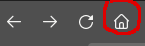
\includegraphics[scale=0.5]{IMG/001--Bouton_accueil.png}
\caption{Bouton d'accès à la page d'accueil}
\end{center}
\end{figure}
\medskip

\paragraph*{La méthode du glisser-déposer:} depuis la barre d'adresse glisser l'adresse de la page \textit{Web} sur le bouton d'accès à la page d'accueil, puis valider ou pas votre choix de définir cette page \textit{Web} comme étant la page d'accueil de \texttt{Firefox}.
\medskip

\paragraph*{Depuis les paramètres:} cliquer sur le bouton d'accès au menu, choisir le \textit{panneau accueil}. Cliquez ensuite sur le menu déroulant à côté de \textit{Page d’accueil et nouvelles fenêtres} puis choisissez d’afficher la \textit{Page d’accueil de Firefox (par défaut)}, des \textit{Adresses web personnalisées...} ou une \textit{Page vide}.
\begin{figure}[h]
\begin{center}

\includegraphics[scale=0.5]{IMG/002--Bouton_menu.png}
\caption{Bouton d'accès au menu}
\end{center}
\end{figure}
\medskip

\section{La barre d'adresse}
\subsection*{Rechercher avec la barre d'adresse}
La barre d’adresse vous permet de trouver facilement ce que vous recherchez. Saisissez-y quelques mots ou une adresse web pour obtenir des suggestions pour votre recherche prises parmi vos sites web les plus visités, vos marque-pages, votre historique ou bien fournies par vos moteurs de recherche – tout cela au même endroit. 
\medskip

Quand vous menez une recherche depuis la barre d’adresse, c’est votre moteur de recherche par défaut qui est utilisé.
\medskip

Quand vous saisissez le caractère \texttt{@} dans la barre d’adresse, une liste des raccourcis des moteurs de recherche disponibles qui commencent par \texttt{@} est affichée. Vous pouvez en sélectionner un en appuyant sur la touche \texttt{[↓]} ou en cliquant dessus.
\medskip
 
\subsection*{L'autocomplétion}
La barre d’adresse de \texttt{Firefox} affiche l’adresse \textit{web} (l’\textit{URL}) de la page que vous consultez. Quand vous saisissez du texte ou une \textit{URL} dans ce champ, \texttt{Firefox} propose des pages que vous avez déjà visitées et qu’il a mémorisées pour pouvoir vous les suggérer dans le panneau qui se déploie sous la barre d’adresse, comme les sites que vous avez marqués, étiquetés, simplement visités ou ouverts dans des onglets.
\medskip

Une icône d’étoile bleue indique que le résultat correspondant est un marque-page; le texte \og \texttt{Aller à l’onglet}\fg{} indique qu’il s’agit d’un onglet ouvert. Si vous voyez la page recherchée, il vous suffit soit de cliquer dessus, soit d’utiliser les flèches vers le haut ou vers le bas de votre clavier pour la mettre en surbrillance puis d’appuyer sur la touche \texttt{<Entrée>}.
\medskip

La barre d’adresse apprend également de votre comportement de navigation, comme la fréquence et la récence de visite de chaque page, ou encore la suggestion sur laquelle vous avez cliqué après la saisie de quelques caractères ou mots. De cette façon, les pages que vous consultez très fréquemment s’affichent en haut de liste, souvent après n’avoir saisi qu’un seul caractère.
\medskip

\paragraph{Paramétrer les résultats montrés par la barre d'adresse:} désactiver l'autocomplétion ou la restreindre.
\begin{verbatim}
    Menu > Paramètres > Vie privée et sécurité > Barre d'adresse
\end{verbatim}
\medskip

Sélectionner ou désélectionner les options du tableau ci-dessous:
\begin{table}[!h]
\begin{center}
\begin{tabular}{|p{4.5cm}|p{7cm}|}
\hline
\textbf{Option} & \textbf{Son action} \\
\hline
L’historique de navigation  & Suggère des pages que vous avez consultées précédemment. \\
\hline
Les marque-pages & Suggère des pages que vous avez marquées précédemment. \\
\hline
Les onglets ouverts & Suggère des pages que vous avez ouvertes dans d’autres onglets. \\
\hline
Les raccourcis & Suggère les sites que vous avez le plus visités (si cette option est choisie dans le panneau Accueil). \\
\hline
Les moteurs de recherche & Suggère d’effectuer une recherche avec un de vos moteurs. \\
\hline  
\end{tabular}
\caption{Options d'autocomplétion de la barre d'adresse}
\end{center}
\end{table}
\medskip

Si vous voulez supprimer tous les résultats d’historique de la liste d’autocomplétion supprimez l’historique de navigation de \texttt{Firefox}.
\medskip

\paragraph*{Cibler les résultats d'autocomplétion} à l'aide des caractères spéciaux du tableau ci-dessous:
\begin{table}[!h]
\begin{center}
\begin{tabular}{|p{3.5cm}|p{8.5cm}|}
\hline
\textbf{Caractère spécial} & \textbf{Action} \\
\hline
\texttt{\^} & pour montrer seulement des correspondances dans votre historique de navigation. \\
\hline
\texttt{*} & pour montrer seulement des correspondances dans vos marque-pages. \\
\hline
\texttt{+} & pour montrer seulement des correspondances dans les pages que vous avez étiquetées. \\
\hline
\texttt{\%} & pour montrer seulement des correspondances dans les onglets actuellement ouverts. \\
\hline
\texttt{\#} & pour montrer seulement des correspondances où chaque terme de la recherche figure dans les titres de page ou dans l’étiquette. \\
\hline
\texttt{\$} & pour montrer seulement des correspondances où chaque terme de la recherche figure dans l’adresse \textit{web} (\textit{URL}). Le texte \texttt{https://} ou \texttt{http://} dans l’\textit{URL} est ignoré, mais non \texttt{file:///}. \\
\hline
\texttt{?} & pour montrer seulement les suggestions de recherche. \\
\hline 
\end{tabular}
\caption{Caractères spéciaux pour cibler l'autocomplétion}
\end{center}
\end{table}
\medskip
 
\section{Navigation par onglets}
\section{Recherche dans les documents}
Avec \texttt{Firefox}, vous pouvez rechercher des mots ou des phrases apparaissant dans la page. \texttt{Firefox} vous montre le prochain endroit où votre recherche apparaît dans la page et vous permet de surligner toutes les occurrences de votre recherche.
\medskip

\subsection*{Avec la barre de recherche}
Pour rechercher du texte sur une page
\begin{verbatim}
    Menu -> Rechercher dans la page...
\end{verbatim}
\medskip

Ou bien: \texttt{[Ctrl]} + \texttt{[F]}
\medskip

Une barre de recherche apparaît au bas de la fenêtre.
\begin{figure}[!h]
\begin{center}

\includegraphics[scale=0.3]{IMG/005--Barre_recherche.png}
\caption{Barre de recherche}
\end{center}
\end{figure}
\medskip

\subsection*{Recherche rapide}
Appuyez sur la touche \texttt{/} (barre oblique) en dehors d’un champ de saisie pour ouvrir la barre de recherche rapide. Saisissez alors ce que vous voulez rechercher.
\medskip

\subsection*{Recherche de lien seulement}
Appuyez sur la touche \texttt{'} (apostrophe) en dehors d’un champ de saisie pour faire apparaître la barre \og Recherche rapide (liens seulement)\fg{}. Saisissez une expression dans le champ de la barre de recherche rapide. Le premier lien contenant l’expression entrée sera sélectionné. 
\medskip

\section{Avec les fichiers \texttt{.pdf}}
\texttt{Firefox} dispose d’une visionneuse \textit{PDF} (\textit{Portable Document Format}) intégrée qui permet l’affichage des fichiers au format \textit{PDF} dans la fenêtre du navigateur. La visionneuse intégrée est utilisée lorsque les fichiers \textit{PDF} sont réglés sur \texttt{Ouvrir dans Firefox} dans les paramètres de gestion des types de fichiers de \texttt{Firefox}. Il s’agit du réglage par défaut. La visionneuse \textit{PDF} intégrée ouvre le fichier \textit{PDF} dans \texttt{Firefox} sans l’enregistrer. Vous pouvez utiliser le bouton de téléchargement présent dans la barre d’outils de la visionneuse pour le télécharger et l’enregistrer\footnote{Pour une utilisation détaillée de la visionneuse intégrée, voir \url{https://support.mozilla.org/fr/kb/voir-fichiers-pdf-firefox-ou-choisir-autre-visionneuse#w_utiliser-la-visionneuse-integree-de-firefox}}.
\begin{figure}[!h]
\begin{center}
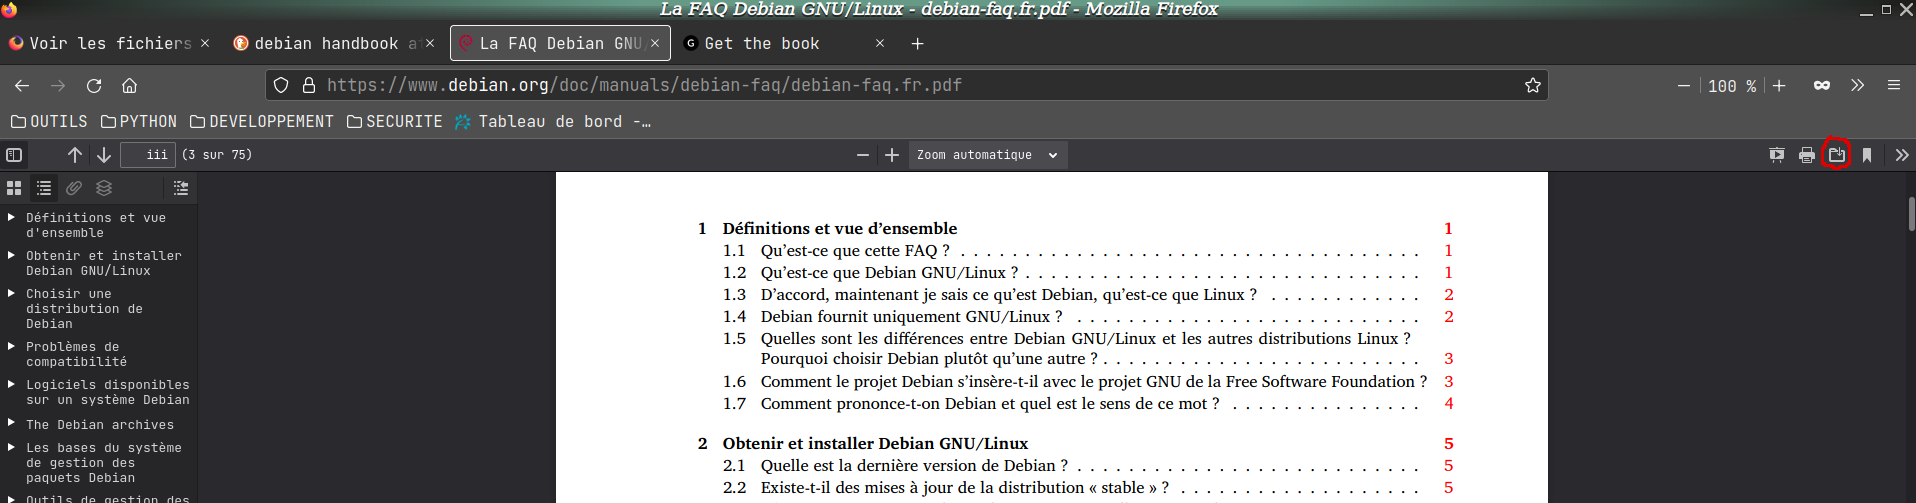
\includegraphics[scale=0.2]{IMG/006--Visionneuse_pdf.png}
\caption{La visionneuse \textit{PDF} intégrée et le bouton de téléchargement}
\end{center}
\end{figure}
\medskip

Pour visualiser le fichier dans une autre visionneuse, se  rendre dans l'historique des téléchargements (Cf. la gestion des téléchargements, page \pageref{Telecharge}), clic droit sur le fichier et sélectionner \texttt{Ouvrir avec} et choisir la visionneuse désirée.
\medskip

\subsection*{Choisir d'utiliser une autre visionneuse par défaut}
\begin{verbatim}
    Menu > Paramètres > Général > (descendre jusqu'à) Applications
\end{verbatim}
\medskip

Sélectionnez dans la liste \texttt{Portable Document Format (PDF)} et cliquez pour sélectionner votre visionneuse dans le menu déroulant qui s'ouvre.
\medskip

\section{Les marque-pages}
Les marque-pages sont des liens vers des pages \textit{Web} qui facilitent le retour à vos endroits favoris.
\medskip

\subsection*{Marquer une page}
Pour marquer une page, il suffit de cliquer sur l’étoile dans la barre d’adresse. 
\begin{figure}[!h]
\begin{center}
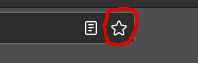
\includegraphics[scale=0.5]{IMG/007--Marque_page.png}
\caption{Marquer une page}
\end{center}
\end{figure}
\medskip

Ou bien pressez les touches \texttt{[Ctrl]} + \texttt{[D]}.
\medskip

L’étoile devient bleue quand la page est marquée et une fenêtre apparaît pour que vous puissiez donner un nom à votre marque-page, en changer l’emplacement ou l’étiqueter. 
\medskip

Marquer tous les onglets ouverts en une opération : effectuez un clic droit sur n’importe lequel des onglets, choisissez \texttt{Sélectionnez tous les onglets...} dans le menu contextuel, puis effectuez un clic droit sur n’importe lequel des onglets et sélectionnez \texttt{Marquer ces onglets...}. Donnez un nom au nouveau dossier contenant ces marque-pages et choisissez le dossier dans lequel vous allez le ranger.
\medskip

\subsection*{Changer le nom d’un marque-page ou son emplacement}
Pour modifier les détails de votre marque-page, cliquez sur l’étoile une deuxième fois pour ouvrir la boîte de dialogue \texttt{Modifier le marque-page}. Vous pouvez alors modifier le nom, l'emplacement ou les étiquettes.
\medskip

\subsection*{Retrouver ses marque-pages}
\paragraph*{Recherche dans la barre d’adresse:}vous pouvez rechercher une page que vous avez marquée en saisissant son nom dans la barre d’adresse. Au fur et à mesure de votre saisie, s’affiche une liste de pages web que vous avez marquées, étiquetées ou visitées. Les pages marquées sont repérées par une étoile devant leur nom. 
\medskip

\paragraph*{La barre personnelle}de \texttt{Firefox} procure un accès rapide aux marque-pages que vous utilisez fréquemment.
\medskip

\paragraph*{Par le menu:}
\begin{verbatim}
    Menu -> Marque_pages
\end{verbatim}
\medskip

\paragraph{Ajouter le bouton \og Menu des marque-pages\fg{} à la barre d’outils:}par défaut, le bouton de menu des marque-pages n’est pas présent dans la barre d’outils mais vous pouvez l’y ajouter en personnalisant la barre d’outils de \texttt{Firefox}\footnote{Voir comment personnaliser la barre d'outils page \pageref{barre_outils}}.
\medskip

\subsection*{Organiser les marque-pages}
La fenêtre \texttt{Bibliothèque} vous permet d’afficher et d’organiser vos marque-pages. Pour ouvrir la fenêtre \texttt{Bibliothèque}:
\begin{verbatim}
    Menu -> Marque-pages -> Organiser les marque-pages (situé au bas du 
    menu)
\end{verbatim} 
\medskip

Ou bien: \texttt{[Ctrl]} + \texttt{[Shift]} + \texttt{[O]}.
\medskip

\begin{figure}[!h]
\begin{center}
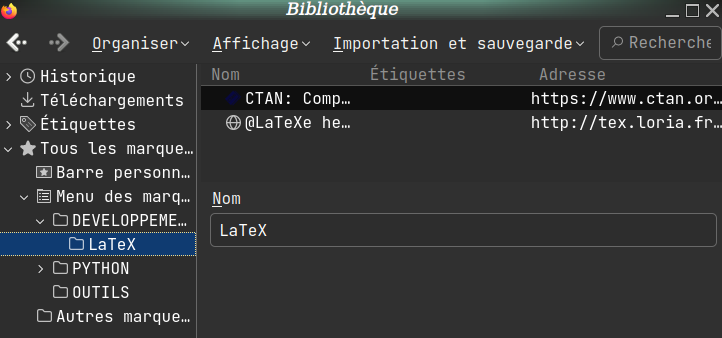
\includegraphics[scale=0.5]{IMG/008--Bibliotheque.png}
\caption{La bibliothèque des marque-pages}
\end{center}
\end{figure}
\medskip

\section{Gestion des fichiers téléchargés}
\subsection*{Historique des téléchargements}
\label{Telecharge}
Pour consulter l'historique des téléchargements:
\begin{verbatim}
    Menu -> Téléchargements
\end{verbatim}
\medskip

Ou \texttt{[Ctrl]} + \texttt{[Shift]} + \texttt{[Y]}
\medskip

\begin{figure}[!h]
\begin{center}
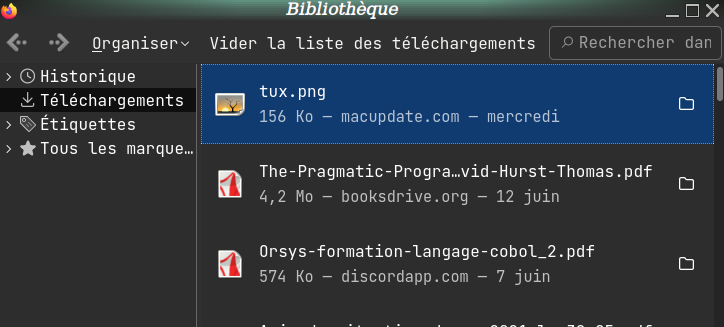
\includegraphics[scale=0.5]{IMG/004-Telechargement.png}
\caption{Historique des téléchargements}
\end{center}
\end{figure}
\medskip

Les téléchargements peuvent être mis en pause ou tout simplement arrêtés.
\medskip

\subsection*{Types de fichiers et actions de téléchargement}
Quand vous cliquez sur un lien pour télécharger un fichier, il se peut que vous voyiez une fenêtre vous demandant si vous voulez enregistrer le fichier ou l’ouvrir avec une application particulière dans les cas où aucune action de téléchargement n’a été définie pour les fichiers de ce type.
\medskip

\subsection*{Changer les actions de téléchargement}
\begin{verbatim}
    Menu > Paramètres > Général > Applications
\end{verbatim}
\medskip

\begin{figure}[!h]
\begin{center}
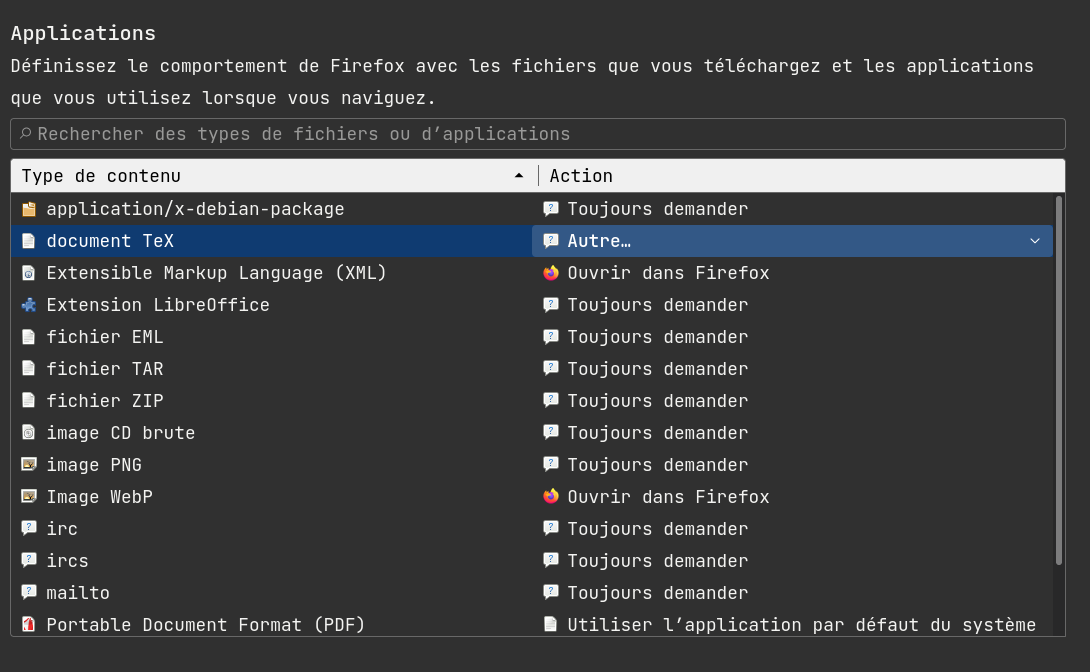
\includegraphics[scale=0.37]{IMG/009--Telechargement.png}
\caption{Modifier les actions de téléchargement selon le type de fichiers}
\end{center}
\end{figure}
\medskip

\begin{table}[!h]
\begin{center}
\begin{tabular}{|p{2.5cm}|p{9.5cm}|}
\hline
\textbf{Action} & \textbf{Description} \\
\hline
Ouvrir dans \texttt{Firefox} & Choisir cette option si vous souhaitez que ce soit \textit{Firefox} qui affiche ce contenu. Cela ne concerne qu’un nombre limité de types de contenu, ceux que \textit{Firefox} peut décoder (\texttt{PDF}, \texttt{XML}, \texttt{SVG} ou Image \texttt{WebP}).\\
\hline
Toujours demander & Affiche une invite demandant \texttt{Que doit faire Firefox avec ce fichier ?} afin que vous puissiez choisir l’action que doit prendre \texttt{Firefox}. Cela peut se révéler utile quand \texttt{Firefox} sauvegarde automatiquement les fichiers d’un type donné ou les ouvre systématiquement avec la même application, alors que vous souhaitez choisir au coup par coup l’action à appliquer.\\
\hline
Enregistrer le fichier & Enregistre toujours le fichier dans votre ordinateur, quand vous téléchargez un fichier de ce type.\\
\hline
Utiliser l’application par défaut du système & Ouvre le fichier avec l’application par défaut configurée dans votre système d’exploitation. Cette option n’est montrée que pour les types de contenu qui proposent l’option \texttt{Ouvrir dans Firefox} (\texttt{PDF}, \texttt{XML}, \texttt{SVG} et Image \texttt{WebP}) et que si votre système dispose d’une autre application paramétrée pour ouvrir par défaut les fichiers de ce type.\\
\hline
Utiliser <nom d’une application> & Ouvre le fichier ou gère le protocole avec l’application indiquée.\\
\hline
Autre... & Ouvre la fenêtre \texttt{Choisir une application externe} où vous pouvez choisir l’application que vous souhaitez utiliser.\\
\hline
Détails de l’application... & Si des applications \textit{web}, ou si des applications installées autres que celle par défaut du système sont énumérées, ouvre une fenêtre vous permettant de connaître l’emplacement de ces applications et de supprimer une application comme option disponible.\\
\hline 
\end{tabular}
\caption{Les actions de téléchargement}
\end{center}
\end{table}
\medskip

\subsection*{Ajouter des actions de téléchargement}
Lorsque vous cliquez sur un lien et que \texttt{Firefox} n’a ni type de contenu défini ni action de téléchargement configurée pour ce type de fichiers, \texttt{Firefox} vous demande comment gérer le fichier en affichant une invite. Cette invite apparaît aussi quand l’action de téléchargement est définie à \texttt{Toujours demander} dans les paramètres \texttt{Applications} de \texttt{Firefox}. 
\medskip

\begin{table}[!h]
\begin{center}
\begin{tabular}{|p{2.5cm}|p{9.5cm}|}
\hline
\textbf{Action} & \textbf{Description}\\
\hline
\texttt{Ouvrir avec Firefox} & Ouvre le fichier dans \texttt{Firefox}. Cette option n’est montrée que pour les types de contenu qui contiennent l’option \texttt{Ouvrir dans Firefox} dans la section \texttt{Applications} des paramètres de \texttt{Firefox} (\texttt{PDF}, \texttt{AVIF}, \texttt{XML}, \texttt{SVG} ou Image \texttt{WebP}).\\
\hline
\texttt{Ouvrir avec} & Enregistre le fichier dans un dossier temporaire et l’ouvre dans l’application par défaut du système d’exploitation pour ce type de fichiers (vous pouvez aussi utiliser le menu déroulant pour choisir une autre application).\\
\hline
\texttt{Enregistrer le fichier} & Enregistre le fichier dans le dossier \texttt{Téléchargements} (spécifié dans la section \texttt{Téléchargements} du panneau \texttt{Général} des paramètres de \texttt{Firefox}).\\
\hline
\texttt{Toujours effectuer cette action pour ce type de fichier} & Cocher cette option pour toujours effectuer l’action sélectionnée, puis cliquer sur \texttt{OK}. Cela ajoute une nouvelle entrée à la liste des types de contenu des actions de téléchargement.\\
\hline  
\end{tabular}
\caption{Ce que doit faire \texttt{Firefox} selon le type de fichier.}
\end{center}
\end{table}
\medskip

L’invite \texttt{Que doit faire Firefox avec ce fichier ?} peut n’afficher aucune application par défaut pour quelques types de fichiers que vous téléchargez. Vous pouvez cliquer sur le bouton \texttt{Parcourir...} pour choisir une application installée sur votre ordinateur pour ouvrir le fichier.
\medskip

\subsection*{Réinitialiser les actions de téléchargement pour tous les types de contenu}
Si vous rencontrez des problèmes avec la façon dont \texttt{Firefox} gère les téléchargements de fichiers et que vous n’arrivez pas à les résoudre, ou si, simplement, vous voulez repartir de zéro, vous pouvez restaurer les types de contenu et les actions par défaut en réinitialisant \texttt{Firefox}.
\medskip

\section{Enregisrer une page \textit{Web}}
\texttt{Firefox} vous permet d'enregistrer une page \textit{Web} sur votre ordinateur afin que vous puissiez la lire, sans être connecté à Internet.
\begin{verbatim}
    Menu -> Enregistrer sous...
\end{verbatim}
\medskip

Ou bien: \texttt{[Ctrl]} + \texttt{[S]}
\medskip

Dans la fenêtre de dialogue, saisir un nom pour la page que l'on souhaite enregistrer et choisir un emplacement. Dans le coin en bas à droite de la fenêtre de dialogue, choisir un type de ficher dans le menu déroulant:
\begin{description}
	\item[\texttt{Page \textit{Web} complète}]: enregistre la totalité de la page avec ses images. Cela permet de la visualiser la page telle que l'originale avec les images, mais peut ne pas conserver la structure des liens HTML de la page originale. \texttt{Firefox} crée un nouveau répertoire pour enregistrer la page, les images et tout autre fichier nécessaire à l'affichage complet de la page.
	\item[\texttt{Page \textit{Web}, HTML uniquement}]: enregistre la page originale sans les images. Ce choix préserve la structure HTML originale des liens dans un fichier.
	\item[\texttt{Fichiers texte}]: enregistre la page originale dans un fichier texte. Ce choix ne préserve pas la structure HTML originale des liens, mais vous permet d'afficher une version texte de la page dans n'importe quel éditeur de texte. 
	\item[\texttt{Tous les fichiers}]: cette option est équivalente à l'option \og Page \textit{Web}, HTML uniquement\fg{} mais vous pouvez spécifier une extension au fichier (par exemple \texttt{.htm} ou \texttt{.shtml}). 
\end{description}
\medskip

\section{Le correcteur orthographique de \texttt{Firefox}}
\texttt{Firefox} vérifie automatiquement l’orthographe des mots que vous écrivez dans les zones de texte. Dès que vous finissez de saisir le mot, celui-ci est comparé aux termes figurant dans le dictionnaire installé. Si le mot n’est pas dans le dictionnaire, il sera souligné en rouge.
\medskip

\subsection*{Corriger les mots mal orthographiés}
Quand la vérification orthographique est activée, vous pouvez facilement corriger les mots mal orthographiés. Pour corriger le mot mal orthographié, faites un clic droit dessus et sélectionnez l’un des mots suggérés en haut du menu déroulant qui apparaît.
\medskip

Si aucun des mots suggérés ne semble convenir, vous devez le modifier manuellement. Si vous êtes sûr que le mot est orthographié correctement, vous pouvez l’ajouter au dictionnaire. Pour ajouter un mot au dictionnaire sélectionnez \texttt{Ajouter au dictionnaire}. Notez que les mots ajoutés s’appliquent à tous vos dictionnaires.
\medskip

Il est possible d'ajouter des dictionnaires ou de changer de dictionnaire en sélectionnant \texttt{Langues} du même menu déroulant.
\medskip

\subsection*{Supprimer un mot que vous avez accidentellement ajouté}
Il va falloir passer par le répertoire \textit{profil}:
\begin{verbatim}
    menu > Aide > Plus d’informations de dépannage
\end{verbatim}
\medskip

L’onglet \texttt{Informations de dépannage} s’ouvre. Sous la section \texttt{Paramètres de base de l’application}, au niveau de la ligne \texttt{Répertoire de profil}, cliquez sur le bouton \texttt{Ouvrir le répertoire correspondant}. Votre répertoire de profil s’ouvre alors.
\medskip

Ouvrez le fichier \texttt{persdict.dat} dans un éditeur de texte. Chaque mot ajouté se situe sur une ligne séparée. Supprimez la ligne qui contient le mot que vous souhaitez supprimer. Sauvegardez votre travail et quittez l'éditeur. Notez  que les mots sont supprimés pour tous vos dictionnaires.
\medskip
 
\subsection*{Désactiver la vérification automatique de l’orthographe}
\begin{verbatim}
    menu > Paramètres > Général > section Langue 
\end{verbatim}
\medskip

Décochez \texttt{Vérifier l’orthographe pendant la saisie}.
\medskip

\chapter{Préférences}
\section{Les options}
\section{\texttt{about:config}}

\chapter{Les extensions}
Les modules complémentaires sont comme des applications que vous pouvez installer pour que \texttt{Firefox} fonctionne comme vous voulez. Ils sont souvent produits par des développeurs tiers.
\begin{verbatim}
    Bouton 'Menu' > Extensions et thèmes > Recommandations
\end{verbatim}
\medskip

Une fois votre extension choisie, cliquer sur \texttt{Installer le thème} ou \texttt{Ajouter à Firefox}.
\medskip

En bas de la liste des modules complémentaires recommandés, il y a aussi un bouton \texttt{Découvrir davantage de modules} sur lequel vous pouvez cliquer. Il vous conduit au site \textit{addons.mozilla.org}\footnote{\url{https://addons.mozilla.org/fr/firefox/}} où vous pouvez rechercher des modules complémentaires précis. 
\medskip

\section{Extensions en navigation privée}
Une extension qui s’exécute dans les fenêtres de navigation privée peut poser problème si elle a accès à des informations que vous préféreriez garder privées. \texttt{Firefox} vous permet de décider quelles extensions peuvent s’exécuter en navigation privée. En outre, les extensions ne sont plus automatiquement autorisées à s’exécuter en navigation privée, vous devez leur accorder explicitement cette permission, soit à l’installation, soit plus tard dans les paramètres de l’extension.
\medskip

\subsection*{Activer ou désactiver les extensions dans les fenêtres de navigation privée}
\begin{verbatim}
    Menu -> Extensions et thèmes ([Ctrl]+[Shift]+[A]) -> Extensions
\end{verbatim}
\medskip

Dans le panneau ouvert vous pouvez gérer les autorisations des extensions à partie de l'onglet \texttt{Détails} de l'extension.
\medskip

\chapter{Vie privée}
\section{Bloquer les nouvelles demandes d’activation des notifications.}
Si un site indique à \texttt{Firefox} qu’il souhaite afficher des notifications\footnote{Les notifications \textit{Web Push} dans \texttt{Firefox}: \url{https://support.mozilla.org/fr/kb/notifications-web-push-firefox}}, par défaut, \texttt{Firefox} demande si vous voulez en accorder la permission. Vous pouvez paramétrer \texttt{Firefox} de façon à refuser automatiquement la permission sans rien demander. Même après cette modification, vous pouvez ajouter des exceptions pour des sites dont vous souhaitez recevoir les notifications ou utiliser les fonctionnalités \textit{push}.
\begin{verbatim}
    Bouton 'Menu' > Paramètres > Vie privée et sécurité 
\end{verbatim} 
\medskip

Descendez jusqu’à la section \texttt{Permissions}, cliquez sur le bouton \texttt{Paramètres...} correspondant à \texttt{Notifications}. Cochez la case \texttt{Bloquer les nouvelles demandes d’activation des notifications} puis cliquer sur le bouton \texttt{Enregistrer les modifications}.
\medskip

\chapter{Outils aux développeurs}

\chapter{Raccourcis clavier}
\begin{center}
\begin{tabular}{|c|l|}
\hline
\textbf{Raccourcis} & \textbf{Description} \\
\hline
\texttt{[Ctrl] + [F]} & Ouvre la barre de recherche \\
\hline
\texttt{[/]} & Ouvre la barre de recherche rapide \\
\hline
\texttt{[']} & Barre de recherche rapide de lien \\
\hline
\texttt{[Ctrl] + [G]} ou \texttt{[F3]} & Se rendre à l’occurrence suivante de la recherche \\
\hline
\texttt{[Ctrl] + [Shift] + [G]} & Se rendre à l’occurrence précédente de la recherche \\
\hline
\texttt{[Ctrl] + [Shift] + [Y]} & Pour accéder à l'historique des téléchargements \\
\hline
\texttt{[Ctrl] + [S]} & Enregistrer une page \textit{Web} \\
\hline
\end{tabular}
\end{center}

\end{document}